%------------------------------------------------------------------------------
% Author(s):
% Varaun Ramgoole
% Copyright:
%  Copyright (C) 2020 Brad Bachu, Arjun Mohammed, Nicholas Sammy, Kerry Singh
%
%  This file is part of Applied-Mathematics-Unit2 and is distributed under the
%  terms of the MIT License. See the LICENSE file for details.
%
%  Description:
%     Year: 2005 C
%     Module: 1
%     Question: 2 
%------------------------------------------------------------------------------
\usetikzlibrary{patterns}

\begin{subquestions}
	
%------------------------------------------------------------------------------
% 2 a -------------------------------------------------------------------------
%------------------------------------------------------------------------------

\subquestion

The objective function is,

\begin{equation}
	P = 300x + 550y \,.
\end{equation}

%------------------------------------------------------------------------------
% 2 b -------------------------------------------------------------------------
%------------------------------------------------------------------------------

\subquestion

The 4 constraints to this problem are, 

\begin{align}
	x & \geq 0 \,, \nn \\
	y & \geq 0 \,, \nn \\
	3x + 5y & \leq 30 \,, \nn \\
	100x + 250y & \leq 1250 \,.
\end{align}

It should also be noted that
\begin{equation}
	100x + 250y \leq 1250 \equiv 2x + 5y \leq 25 \,.
\end{equation}

%------------------------------------------------------------------------------
% 2 c -------------------------------------------------------------------------
%------------------------------------------------------------------------------

\subquestion

The feasible region is shaded in the graph below.

\begin{center}

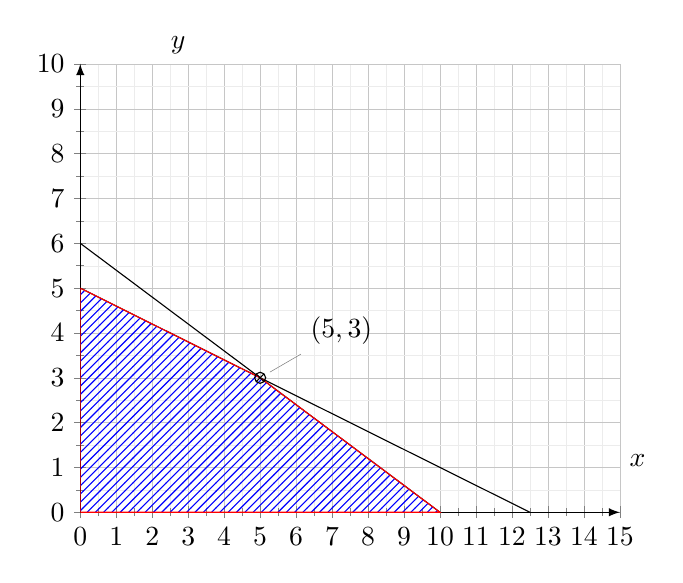
\begin{tikzpicture}
	\begin{axis}
		[
		xmin=-0,xmax=15,
		ymin=0,ymax=10,
		grid=both,
		grid style={line width=.1pt, draw=darkgray!10},
		major grid style={line width=.2pt,draw=darkgray!30},
		axis lines=left,
		minor tick num=1,
		enlargelimits={abs=0},
		axis line style={-latex},
		samples=100,
		domain = -20:20,
		ytick={0,1,...,10},
		xtick={0,1,...,15},
		xlabel={$x$},
		ylabel={$y$},
		x label style={at={(axis description cs:1,0.15)},anchor=north west},
		y label style={at={(axis description cs:0.15,1)},anchor=south west, rotate=-90}
		]
		
		\addplot [mark=dot] coordinates{(10, 0)  (0,6)};
		
		\addplot [mark=dot] coordinates {(12.5,0) (0, 5)};
		
		\addplot [red,pattern=north east lines,pattern color=blue] coordinates {(0,5) (5, 3) (10, 0)} \closedcycle;	
		
		\node [pin=30:{$(5, 3)$}] at (axis cs:(5, 3) {};
		
		\addplot [mark=otimes] coordinates{(5, 3)};
		
	\end{axis}	
\end{tikzpicture}

\end{center}

%------------------------------------------------------------------------------
% 2 d -------------------------------------------------------------------------
%------------------------------------------------------------------------------

\subquestion

From \rdef{mod1:defn:TourOfVertices}, we can calculate $P$ by,

\begin{align}
	\text{Using (0,5)} \,, \nn \\
	P & = 300x + 550y \,, \nn \\
	& = (300 \times 0) + (550 \times 5) \,, \nn \\
	& = 2750 \,.  \\
	\text{Using (5, 3)} \,, \nn \\
	P & = 300x + 550y \,, \nn \\
	& = (300 \times 5) + (550 \times 3) \,, \nn \\
	& = 2550 \,.    \\		  
	\text{Using (10,0)} \,, \nn \\
	P & = 300x + 550y \,, \nn \\
	& = (300 \times 10) + (550 \times 0) \,, \nn \\
	& = 3000 \,. \label{2005:q2:eqn:Profit}
\end{align}

From \req{2005:q2:eqn:Profit}, we see that maximum profit $P$ is $ \$ 3000$.

%------------------------------------------------------------------------------
% 2 e -------------------------------------------------------------------------
%------------------------------------------------------------------------------

\subquestion

The Profit Line method can also be used to determine the maximum value of $P$. It relies on drawing parallel lines, starting from the origin, which have the gradient of the objective function. This line is then drawn at different points on the $x$ or $y$ axes. The furthest point on the feasible region which the Profit Line touches (just before leaving the feasible region) is the point which will yield the maximum value of the objective function. 

\end{subquestions}

